\startcontents[localtoc]
\printcontents[localtoc]{}{0}{\subsection*{Contents}\setcounter{tocdepth}{2}}

\begin{lstlisting}
% Example for algorithm OEFPIL.
\end{lstlisting}


\phantomsection
\addcontentsline{toc}{section}{Generate sample data}
\subsubsection*{Generate sample data}



Set independent and dependent variables for \texttt{OEFPIL} algorithm.

\begin{lstlisting}
DI.x.v = [1 2 3 4 5];
DI.x.u = [0.1 0.1 0.1 0.1 0.1];
DI.y.v = [1.1 1.9 3.1 3.9 5.1];
DI.y.u = [0.1 0.1 0.1 0.1 0.1];

% Suppose the dependence is linear:
DI.exponents.v = [0 1];
\end{lstlisting}


\phantomsection
\addcontentsline{toc}{section}{Call algorithm}
\subsubsection*{Call algorithm}



Use QWTB to apply algorithm \texttt{OEFPIL} to data \texttt{DI}.

\begin{lstlisting}
DO = qwtb('OEFPIL', DI);
\end{lstlisting}
\begin{lstlisting}[language={},xleftmargin=5pt,frame=none]
QWTB: no uncertainty calculation

\end{lstlisting}


\phantomsection
\addcontentsline{toc}{section}{Display results}
\subsubsection*{Display results}



Results is

\begin{lstlisting}
disp(['offset          : ' num2str(DO.coefs.v(1)) ' +- ' num2str(DO.coefs.u(1))])
disp(['linear coeff.   : ' num2str(DO.coefs.v(2)) ' +- ' num2str(DO.coefs.u(2))])
\end{lstlisting}
\begin{lstlisting}[language={},xleftmargin=5pt,frame=none]
offset          : 0.012791 +- 0.46984
linear coeff.   : 1.0024 +- 0.14168

\end{lstlisting}


\phantomsection
\addcontentsline{toc}{section}{Interpolate values}
\subsubsection*{Interpolate values}



Interpolate fitted polynom at values \texttt{t}.

\begin{lstlisting}
t = [0:0.1:6];
ty = DO.func.v(t, DO.coefs.v);

% Calculate uncertainties of interpolated values (|S| is sensitivity matrix, |CC| is covariance
% matrix of coefficients, |CT| is covariance matrix of interpolated values, |uty| is uncertainty of
% interpolated values).
for i = 1:length(t);
        S = t(i).^DI.exponents.v;
        CC = diag(DO.coefs.u,0)*DO.coefs.c*diag(DO.coefs.u,0);
        CT(i)=S*CC*S';
end
uty=CT.^0.5;
\end{lstlisting}


\phantomsection
\addcontentsline{toc}{section}{Plot results}
\subsubsection*{Plot results}

\begin{lstlisting}
figure
hold on
errorbar(DI.x.v, DI.y.v, DI.y.u, 'xb')
errorbar(t, ty, uty, 'og')
plot(t, ty, '-r');
plot(t, ty + uty, '-r');
plot(t, ty - uty, '-r');
xlabel('independent variable')
ylabel('dependent variable')
legend('original data','interpolated values','fit', 'uncer. of int. val.','location','southeast')
hold off
\end{lstlisting}
\begin{center}
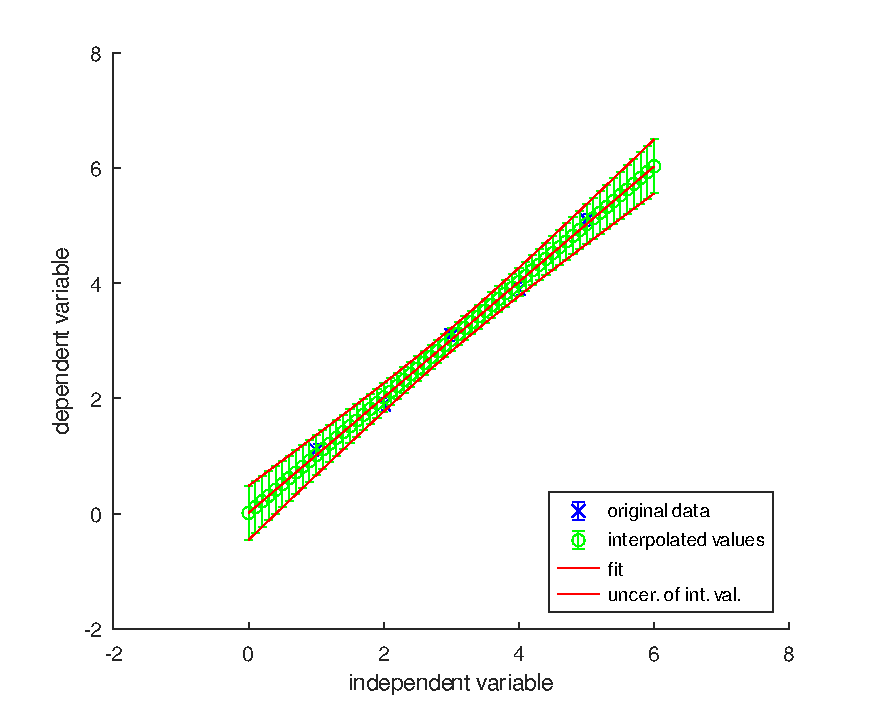
\includegraphics[width=0.7\textwidth]{algs_examples_published/OEFPIL_alg_example-1.pdf}
\end{center}


\stopcontents[localtoc]
